%! Author = joels
%! Date = 24/12/2020

\section{STL Algorithms}
% You know when and why to prefer standard algorithms over hand written loops
% You can name the most important algorithms in the STL
% You can explain certain pittfalls when using STL algorithms
% You can explain the signature of a standard algorithm
% You can write programs that correctly use standard algorithms

Why should we use Algorithms?
\begin{itemize}
    \item Correctness: It is much easier to use an algorithm correctly than implementing loops correctly
    \item Readability: Applying the correct algorithm expresses your intention much better than a loop
    \item Performance: Algorithms might perform better than handwritten loops
\end{itemize}
\subsection{Functor}
A functor is a type (class) that provides a call operator: operator().
\begin{lstlisting}[style=frame, style= linenumbers, language=C]
struct Accumulator {
    int count{0};
    int accumulatedValue{0}
    void operator()(int value) {
        count++;
        accumulatedValue += value;
    }
    int average() const; // To implement
    int sum() const;
};

int average(std::vector<int> values) {
    Accumulator acc{};
    return std::for_each(begin(values), end(values), acc).average();
}
\end{lstlisting}

\subsubsection{Standard Functor Template Classes $\rightarrow$ \#include $<$functional$>$}
\begin{lstlisting}[style=frame, style= linenumbers, language=C]
// Lambda to transform
transform(v.begin(), v.end(), v.begin(), [](int x){ return -x;} );
// Standard Library's Functor: std::negate
transform(v.begin(), v.end(), v.begin(), std::negate<int>{} );
// Sorting with Standard Library Funcor: std::greater
sort(v.begin(), v.end(), std::greater<>{} );
\end{lstlisting}
\subsubsection{Standard Functor Classes $\rightarrow$ \#include $<$functional$>$}
\begin{lstlisting}[style=frame, style= linenumbers, language=C]
// Binary arithmetic and logical            Unary
plus<> (+)                                  negate<> (-)
minus<> (-)                                 logical_not<> (!)
divides<> (/)
multiplies<> (*)                            //Binary comparison
modulus<> (%)                               less<> (<)
logical_and<> (&&)                          less_equal<> (<=)
logical_or<> (||)                           equal_to<> (==)
                                            greater_equal<> (>=)
                                            greater<> (>)
                                            not_equal_to<> (!=)
\end{lstlisting}
\subsection{Algorithm Examples}
\begin{itemize}
    \item transform: Lambda, function or functor for map
    \item merge: ranges must to be sorted
    \item remove/erase: Remove does not actually delete element, it moves the not-removed elements to the front. To get rid of \textit{removed} elements, usually \textit{erease} is called
    \item accumulate: Sums elements that are addable (+ operator)
    \item \_if versions: Take a predicate (instead of value) to provide a condition
    \item \_n versions: algorithm is related to a number (e.g: instead of last iterator)
        \SubItem{\textcolor{blue}{search\_n, copy\_n, fill\_n, generate\_n, for\_each\_n}}
\end{itemize}

\pagebreak

\begin{lstlisting}[style=frame, style= linenumbers, language=C]
// transform
// combined contains: | "ggg" | "" | "u" | "yyyy" | "" | "oo" |
std::vector<int> counts{3, 0, 1, 4, 0, 2};
std::vector<char> letters{'g', 'a', 'u', 'y', 'f', 'o'};
std::vector<std::string> combined{};
auto times = [](int i, char c) { return std::string(i, c); };
std::transform(begin(counts), end(counts), begin(letters), std::back_inserter(combined), times);

// merge
std::vector<int> r1{9, 12, 17, 23, 54, 57, 85, 95};
std::vector<int> r2{2, 30, 32, 41, 49, 63, 72, 88};
std::vector<int> d(r1.size() + r2.size(), 0);
std::merge(begin(r1), end(r1), begin(r2), end(r2), begin(d));

// remove
std::vector<unsigned> values{54, 13, 17, 95, 2, 57, 12, 9};
auto is_prime = []unsigned(u) { /* ... */ };
auto removed = std::remove_if(begin(values), end(values), is_prime);

// accumulate
std::vector<std::string> longMonths {"Jan", "Mar", "May", "Jul", "Aug", "Oct", "Dec"};
std::string accumulatedString = std::accumulate(
    next(begin(longMonths)), // Second element
    end(longMonths), // End
    longMonths.at(0), //First element, usually the neutral element
    [](std::string const & acc, std::string const & element) {
        return acc + ", " + element;
    }); //Jan, Mar, May, Jul, Aug, Oct, Dec

// count_if
std::set<unsigned> numbers{1, 2, 3, 4, 5, 6, 7, 8, 9};
auto isPrime = [](unsigned u) { /* ... */ };
auto nOfPrimes = std::count_if(begin(numbers), end(numbers), isPrime);

// copy_n
std::set<unsigned> numbers{1, 2, 3, 4, 5, 6, 7, 8, 9};
std::vector<unsigned> top5(5);
std::copy_n(rbegin(numbers), 5, begin(top5));
\end{lstlisting}

\subsubsection{Heap Algorithms}
\begin{itemize}
    \item Implementing a binary heap on a sequenced container
    \item Requires random access iterator
    \item Guarantees: Top element is the largest (max), Adding and removing performance guarantees
    \item Used for implementing priority queues
    \item Heap operations: \textcolor{blue}{make\_heap, pop\_heap, push\_heap, sort\_heap}
\end{itemize}
\begin{lstlisting}[style=frame, style= linenumbers, language=C]
// create heap
std::vector<int> v{3, 1, 4, 1, 5, 9, 2, 6}
make_heap(v.begin(), v.end()); // create tree order
// remove largest element
pop_heap(v.begin(), v.end()); // reorder
v.pop_back();
// add element
v.push_back(8);
push_heap(v.begin(), v.end()); // reorder
sort_heap(v.begin(), v.end()); // smallest element first in vector
\end{lstlisting}

\subsection{Algorithm Headers}
\subsubsection{Algorithms in Standard Library}
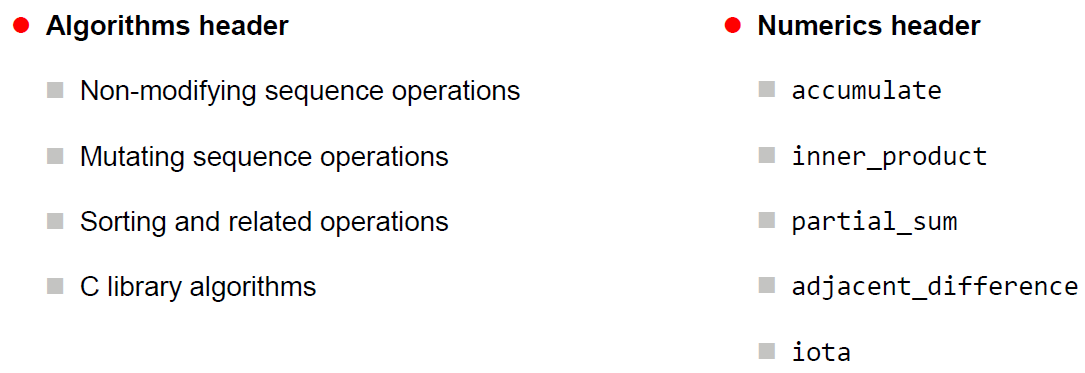
\includegraphics[scale=0.4]{media/algo_header.png}
\subsubsection{Algorithms: Non-Modifying Sequence Operations}
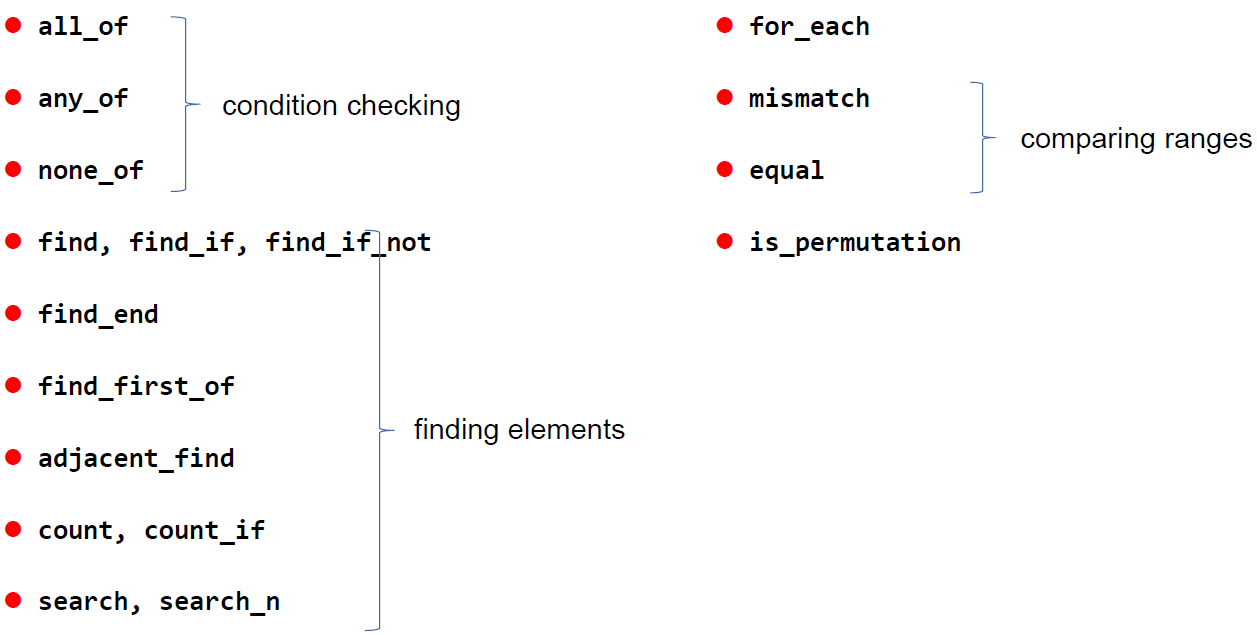
\includegraphics[scale=0.4]{media/algo1.png}
\subsubsection{Mutating sequence operations}
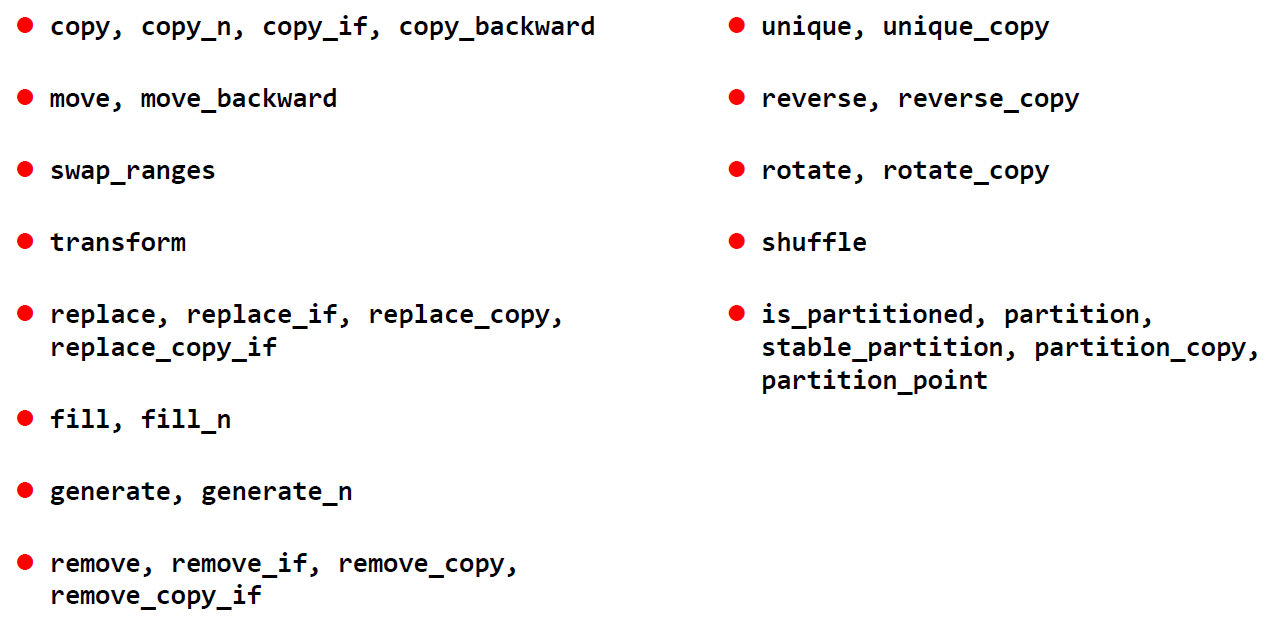
\includegraphics[scale=0.4]{media/algo2.png}
\subsubsection{Algorithms: Sorting and Related Operations}
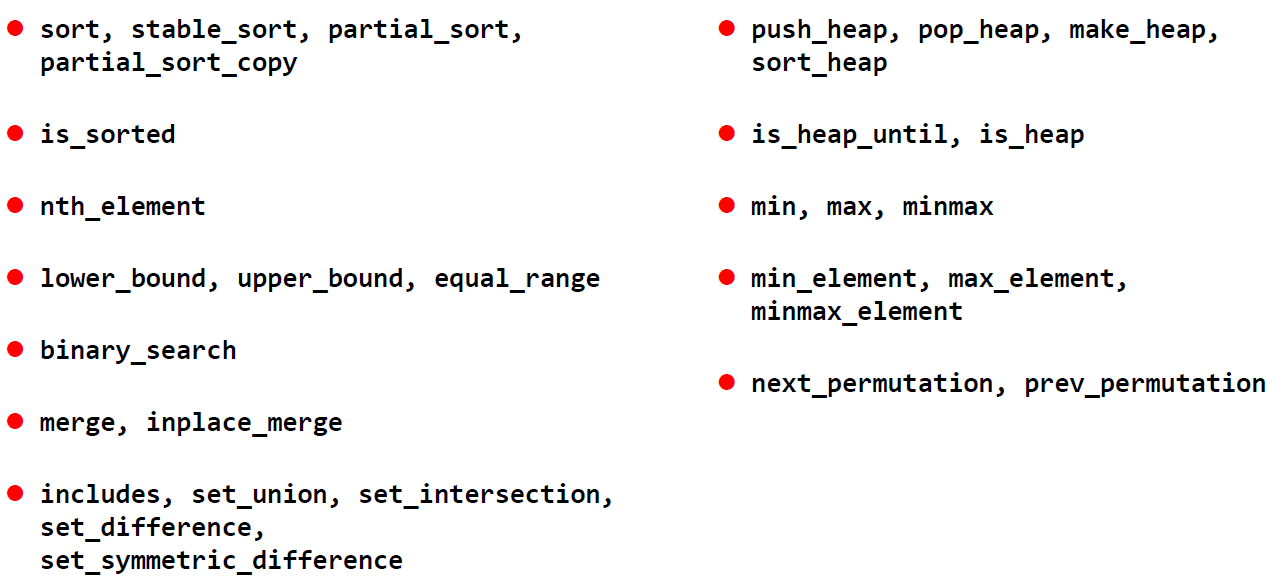
\includegraphics[scale=0.4]{media/algo3.png}